\documentclass[11pt]{amsbook}

\usepackage{geometry}  
\geometry{letterpaper} 
\usepackage{graphicx}
%\usepackage[backend=bibtex]{biblatex}
\usepackage{array}
\usepackage{amssymb}
\usepackage{amsmath}
\usepackage{amsthm}
\usepackage{graphicx}
\usepackage[parfill]{parskip} 
\usepackage[utf8]{inputenc}
\usepackage[english]{babel}
\usepackage{enumerate}
\usepackage{tikz}
\usepackage{tikz-cd}
\usepackage[noend]{algpseudocode}
\usepackage{caption}
\usepackage{subcaption}
\usepackage{fancyhdr}
\usepackage{enumitem}
\usepackage[super]{nth}
\usepackage{pstricks}
\usepackage{xstring}
\usepackage{comment}
\usepackage{pgfplots}
\usepackage{blkarray} %This is for labelled matrices
\usetikzlibrary{decorations.pathreplacing} % this is for Ai's drawing



\usepackage[colorlinks=true,linkcolor=blue]{hyperref}


\pagestyle{fancy}
\lhead{}
\chead{}
\rhead{}
\lfoot{}
\cfoot{\thepage}
\rfoot{}
\renewcommand{\headrulewidth}{0pt}
\setlength{\footskip}{50pt}

\makeatletter
\def\BState{\State\hskip-\ALG@thistlm}
\makeatother

\theoremstyle{plain}
\newtheorem{thm}{Theorem}[section]

\newtheorem{cor}[thm]{Corollary}

\newtheorem{prop}[thm]{Proposition}

\newtheorem{dfn}[thm]{Definition}

\newtheorem{lem}[thm]{Lemma}

\newtheorem{ex}[thm]{Example}

\newtheorem{conj}[thm]{Conjecture}

\newtheorem*{rem}{Remark}
\newtheorem{assumption}[thm]{Assumption}

\newcommand{\Rom}[1]
    {\MakeUppercase{\romannumeral #1}}
\newcommand{\C}[1]{(\mathbb{C}^*)^#1}
\newcommand{\ldp}{log del Pezzo}
\newcommand{\mb}[1]{\mathbb{#1}}
\newcommand{\Hi}{Hirzebruch surface }
\newcommand{\minres}{minimal resolution}
\newcommand{\LJ}{Looijenga pair}
\newcommand{\ra}{\rightarrow}
\newcommand{\spl}{\text{SL}_2 (\mathbb{C})}
\newcommand{\gl}{\text{GL}_2 (\mathbb{C})}
\newcommand{\pgl}{\text{PGL}_2 (\mathbb{C})}
\newcommand{\wt}[1]{\widetilde #1}
\newcommand{\Q}{\mathbb{Q}}
\newcommand{\Z}{\mathbb{Z}}
\newcommand{\F}{\mathbb{F}}
\renewcommand{\P}{\mathbb{P}}


\pgfdeclarelayer{edgelayer}
\pgfdeclarelayer{nodelayer}


\pgfsetlayers{edgelayer,nodelayer,main}

% Node styles
\tikzstyle{none} = []
\tikzstyle{Filled Basic}=[fill=black, draw=black, shape=circle]

% Edge styles
\tikzstyle{Dashed Line}=[-, draw=blue, dashed]
\tikzstyle{Filled Blue}=[-, draw=blue]
\tikzstyle{Dashed Black}=[-, draw=black, dashed]
\tikzstyle{Red}=[-, draw={rgb,255: red,191; green,0; blue,64}]
\tikzstyle{new edge style 0}=[-, dashed, draw={rgb,255: red,191; green,0; blue,64}]


\graphicspath{ {images/} }

\begin{document} 

\setcounter{chapter}{2}

\section{Context}
The main result of this chapter is 
\begin{thm}\label{ThmOnSing}
Let $X$ be a non-smooth \ldp\ with only singularities of small discrepancy. Then 
\begin{enumerate}
\item\label{thm38i}
$X$ has either one singularity or two singularities, and if there are two each of them are of type $\frac{1}p(1,1)$ for some, possibly different,~$p$.
\item\label{thm38ii}
If $X$ admits no floating $-1$-curves then $X$ admits a toric degeneration. %In particular given a singularity $S$ we have at most $m$ basic surfaces, where $m$ is the number of exceptional curves in the resolution of $S$.
\end{enumerate}
\end{thm}
\textbf{This is a first draft, context will be inserted}

\section{Standard notions and notation for quotient singularities}
\label{sec!notation}

\section{Singularities with small discrepancy}

Recall from Section~\ref{sec!notation} our standard notation for quotient singularities.
We consider the germ $S$ of a cyclic quotient singularity appearing at a point $P$ on a 
projective surface $X$.
The minimal resolution of $X$ is denoted $f\colon Y \longrightarrow X$. It contains a chain of
exceptional (smooth, rational)
curves $C_1,\dots,C_n$, entirely determined by $S$ itself, which are ordered so
that the only intersections between these curves are
$C_i\cap C_{i+1}$ which is a single transverse intersection for each $i=1,\dots,n-1$; 
in other words,
$C_1$ and $C_n$ are the two `ends' of the chain.
We also denote the discrepancies of each $C_i$ (as curves in $Y$) by $d_i\in\Q$: thus
\[
K_Y = f^*(K_X) + \sum_{i=1}^n d_i C_i.
\]
We introduce a property of cyclic quotient singularities that is central to the rest of the chapter.
\begin{dfn}
Let $S$ be a cyclic quotient singularity, and $C_1, \dots ,C_n$ the exceptional curves of the minimal resolution of $S$ and $d_1, \dots,d_n$ their discrepancies, as above.
We say that $S$ is a \emph{singularity with small discrepancy} if $d_i \leq -\frac{1}{2}$ for
all $i=1,\dots,n$.
\end{dfn}

To simplify our calculations we introduce to the notation $e_i = d_i + 1$. 

\begin{prop}
In the notation above,
a singularity $S$ has small discrepancy if and only if $C_1^2 \neq -2$ and $C_n^2 \neq -2$ and $ S \not\cong \frac{1}{3}(1,1)$.
\end{prop}
\begin{proof}
 We use the fact that the discrepancy is a strictly decreasing sequence then a strictly increasing sequence. So it suffices to show this for $C_1$ and $C_n$ and then apply this to show it for the intermediate values. We use the following formula for the discrepancy $e_i =  \frac{e_{i-1}+e_{i+1}}{a_i}$. We note that if $a_1 \geq 4$, then as $e_0 = 1$ and $e_2 \leq 1$ we have $e_1 \leq \frac{2}{-4}$. This implies the inequality for small discrepancy. In the case where $a_1 = 3$ this results in the following, as $e_1 \geq e_2$ by substituting $e_2$ into $e_1 = \frac{1 + e_2}{-3}$ we get  $ e_2 \leq \frac{1 + e_2}{3}$ rearranges to $2e_2 - 1 < 0$. Hence $e_2 \leq \frac{1}{2}$. Substituting this back into the equation for $e_1$ we get $e_1 \leq  \frac{1+ \frac{1}{2}}{3} =  \frac{1}{2}$. 
 \end{proof}


Throughout the rest of this chapter we restrict the class of singularities we consider as follows:

\begin{assumption}
Any singularity germ $S$ that appears in this chapter is assumed to be a cyclic
quotient singularity with small discrepancy.
\end{assumption}

\section{Log del Pezzo surfaces and small discrepancy}

\begin{dfn}[\cite{Artin}]
Let $X$ be a surface. A $-1$ cycle $Z = \sum_{D \in S} D \subset X$ is a rationally connected set of curves such that there is a sequence of maps 
\[
% https://tikzcd.yichuanshen.de/#N4Igdg9gJgpgziAXAbVABwnAlgFyxMJZABgBpiBdUkANwEMAbAVxiRAA0BedgfWJAC+pdJlz5CKAIzkqtRiza9Jg4SAzY8BIgCYZ1es1aIQAHRMBjKBBwIhIjeKIBmPXMOKehAbJhQA5vBEoABmAE4QALZIZCA4EEiSdiBhkQnUcUjaSSlRiLqx8YhO3gJAA
\begin{tikzcd}
X=X_0 \arrow[r] & X_1 \arrow[r] & \cdots \arrow[r] & X_n
\end{tikzcd}
\]
Such that each map is a contraction of a $-1$ curve $D \in S$ and the image of $Z$ is a nonsingular point.
\end{dfn}

\begin{lem}\label{lem!badcurve}
Let $X$ be a surface having cyclic quotient singularities of small discrepancy, and let  $f \colon Y \rightarrow X$ be the minimal resolution of $X$. Let $C \subset X$ be a rational curve whose 
strict transform $\widetilde C \subset Y$ is smooth. Let $\{ E_i \}$ be the exceptional locus of $f$. Suppose in addition that 
$\widetilde C \cdot \sum E_i \geq 2$.
Then if $\widetilde C^2 = -1$ implies $-K_X \cdot C \leq 0$.

In particular, $\widetilde C$ is smooth and
$C$ either meets at least two singularities of $X$ or meets one singularity
with at least branches or has a singular point of $C$ at a singularity of $X$,
then the hypotheses on $C$ are satisfied.
\end{lem}
\begin{proof}
%Let $f \colon : Y \rightarrow X$ be the minimal resolution of $X$, $\widetilde C \subset Y$ the strict transform of $C$. 
By the genus formula for $\widetilde C\subset Y$, as $\widetilde C$ and $Y$ are both smooth,
$K_Y \cdot \widetilde C = -1$. If $\wt C$ intersects two distinct exceptional curves $E_i$, $E_j$,
with discrepancy $d_i$, $d_j$ respectively, then
 $K_X \cdot C = f^*(K_X) \cdot \widetilde C \geq -1 - d_i - d_j  \geq 0$,
 as $X$ has only singularities with small discrepancy. 
 If, on the other hand, $\wt C$ meets only one exceptional curve $E_i$, but with intersection
multiplicity $m_i$, then $K_X \cdot C = f^*(K_X) \cdot \widetilde C \geq -1 - m_id_i  \geq 0$.
\end{proof}

We show next that in fact such rational curves cannot lie on a \ldp.
We need a preliminary lemma.
\begin{lem}\label{lem!minus2curve}
Let $X$ be a \ldp\ and $f \colon Y \rightarrow X$ its \minres.
Let $C\subset Y$ be a smooth rational curve. If $C^2\le-2$ then $C$ is contracted by $f$
to a point of~$X$.
\end{lem}

\begin{proof}
We proof this by contradiction. Assume there is a curve $C$ that is not contracted. Then 
\[
K_X \cdot f(C) = f^*(K_X) \cdot \wt{C} \geq K_Y \cdot \wt{C} \geq 0
\]
The first inequality follows as $f^*(K_X) - K_Y$ is an effective divisor. The second inequality follows as $K_Y \cdot \wt{C} = -2 - \wt{C}^2$.
\end{proof}

\begin{prop}\label{MainProp}
Let $X$ be a \ldp\ with singularities of small discrepancy and $f \colon Y \ra X$ its minimal resolution.
Consider the following diagram
\[
% https://tikzcd.yichuanshen.de/#N4Igdg9gJgpgziAXAbVABwnAlgFyxMJZARgBoAGAXVJADcBDAGwFcYkQANEAX1PU1z5CKAEyli1Ok1bsAmjz4gM2PASLlxkhizaIQALR6SYUAObwioAGYAnCAFskGkDghIyUnewA63uAGMbLDQcOBwAT0YYYFNuEBpGegAjGEYABQFVYRAg0wALHAVrO0dEZ1ckMU8ZPV8AoJCwyOirOO5KbiA
\begin{tikzcd}
  & Y \arrow[rd, "\scriptstyle{g}"'] \arrow[ld, "\scriptstyle{f}"] &   \\
X &                                                                & Z
\end{tikzcd}
\]
$f$ is the minimal resolution of $X$ and $g$ is a birational morphism to a smooth surface $Z$.
Let $E\subset Y$ be an $f$-exceptional curve. Then either $E$ is contracted to a smooth point
of $Z$ by $g$, or $g(E)$ is a smooth curve and $g_E$ is an isomorphism.
\end{prop}

\begin{proof}
Let $E\subset Y$ be any one of the exceptional curves $E_i^S$ over a singularity $S$ of $X$; in particular, $E$ is
a smooth rational curve with $E^2 \le-2$.
We first show that if $g_* E\subset Z$ is a curve, then it must be a smooth curve. 

For contradiction, suppose $g_*E$ is a curve with a singular point $P$.
Let $C_1,\dots,C_s\subset Y$ be the curves that contract to $P$ under~$g$.
As these curves are contracted, $C_i^2 \leq  -1$.
Notice that if $C_i^2\le-2$, then $f(C_i)$ is a point of~$X$
by Lemma~\ref{lem!minus2curve}.
There are two cases to consider: set-theoretically, either
$g^{-1}(P)$ meets $E$ in a single point or in more than one point.


In the case of more than one intersection point, since $g^{-1}(g_*(E))$ is connected,
among the curves $C_i$ there must be a shortest chain $C_1\cup\cdots\cup C_r$
with $C_k\cdot E=0$ for $k=2,\dots,r-1$, and $\left(\sum_{i=1}^r C_i\right)\cdot E = 2$.
At least one of the curves $A=C_k$ of the cycle must have $A^2=-1$, otherwise the
whole cycle is contracted to a point $R$ of $X$, but then $R\in X$ would not be
a rational singularity, and so in particular not a cyclic quotient singularity.
And of course $A$ cannot meet another $-1$-curve $C_j$ with $g(C_j)=P$.
Thus $A$ must lie in one of the following configurations:
\begin{enumerate}
\item
$A$ meets two distinct $\pi$-exceptional curves, $C_j$ and $C_{j'}$,
both of which have self-intersection $\le-2$.
\item
$A$ meets $E$ in one point and a distinct $\pi$-exceptional curves $C_j$
with $C_j^2\le-2$.
\item
$A$ meets $E$ in two distinct points.
\end{enumerate}
In each of these situations, $C = f_*(A)\subset X$ would be a curve
on which $K_X$ is nef, by Lemma~\ref{lem!badcurve}, which contradicts
$X$ being a \ldp surface. Indeed $A = \wt C$ meets the $f$-exceptional locus with multiplicity
at least~2 in each case.

The argument in the nodal case follows similarly, up to the case division of configurations
at which there is an additional case:

We note that if $g^{-1}{P}$ contains two curve $C_i$, $C_j$ with $I_Q (C_i, \, C_j) \ge 2$ then either one of them is a $-1$-curve or it cannot occur on the minimal resolution of a \ldp\ surface. This is because every curve in $\pi^{-1}{P}$ has negative self-intersection, if its intersection is less than $-1$ then it would have to be contracted on the map down to $X$, resulting in a noncyclic quotient singularity. Hence one of them is $-1$ curve, and this cannot occur as it would contradict Lemma~\ref{lem!badcurve}. Hence this cannot occur, so we have to blow up the point $P$ enough times such that all the intersections are transverse. At this point we have a curve $A$ such that $A$ intersects transversely at least three other curves, $E, \, C_1, \, C_2 \dots $ with $C_i \in \pi^{-1} {P}$. In addition $C$ is the only $-1$ curve in $\pi^{-1}{P}$. As $Y$ is constructed from further blowups we split into configurations 

\begin{enumerate}
\item
The strict transform of $A$, denoted $\widetilde{A}$ has $\wt{A}^2 = -1$.
\item
The strict transform of $A$, denoted $\widetilde{A}$ has $\wt{A}^2 \leq -2$.
\end{enumerate}

In the first case Lemma~\ref{lem!badcurve} this cannot occur on the minimal resolution of a \ldp\ surface due to the curves $\wt{E}, \, \wt{C_1},\, \wt{C_2}$. In the second case, if none of the intersection points $A\cap E, \, A \cap C_1, \, A \cap C_2$ have been blown up then we are left with a noncyclic quotient singularity. Hence one of these points has to be blown up. This results in a $-1$-curve intersecting $\wt{A}$ and another negative curve hence we have a contradiction to Lemma~\ref{lem!badcurve}.


For a completely general curve singularity it follows by a combination of the above arguments. 
\end{proof}


\begin{prop}\label{Surfaces to F_1}
There is a unique family of singular log del Pezzo surfaces $S_p$, indexed by $p \in \mb{N}$, such that given the minimal resolution $Y$ of $S_p$, $Y$ does not admit a map to $\mb{F}_i$ with $i \geq 2$. Here $S_p$ has one $\frac{1}{p}(1,1)$ singularity.
\end{prop}

\begin{proof}

The first case is that $Y$ only admits a map to $\mb{F}_0$. Then $Y$ must be $\F_0$, since a blow up of any point of $\mb{F}_0$ also permits a map to $\mb{F}_1$; but then $X=Y$ is smooth, contradicting the assumption. 

For $\mb{F}_1$ other cases arise. Clearly if we blow up a point on the $-1$-curve we get a map to $\mb{F}_2$. So the only option is a blowup at a smooth point. At this point you get the following toric variety 

\[
\begin{tikzpicture}[scale=0.5]
	\begin{pgfonlayer}{nodelayer}
		\node [style=none] (0) at (-4, 0.25) {};
		\node [style=none] (1) at (0, 4) {};
		\node [style=none] (2) at (-3, 2) {};
		\node [style=none] (3) at (-3, -3) {};
		\node [style=none] (4) at (-2, 3) {};
		\node [style=none] (5) at (3, 3) {};
		\node [style=none] (6) at (2, -3) {};
		\node [style=none] (7) at (3, -2) {};
		\node [style=none] (8) at (-4, -2) {};
		\node [style=none] (9) at (-4, -2) {};
		\node [style=none] (10) at (2, 4) {};
		\node [style=none] (11) at (-1.75, 1.75) {-1};
		\node [style=none] (12) at (0.25, 2.75) {};
		\node [style=none] (13) at (0.25, 2.55) {-1};
		\node [style=none] (14) at (1.5, 0.75) {0};
		\node [style=none] (15) at (-0.5, -1.5) {0};
		\node [style=none] (16) at (-2.5, -0.25) {-1};
	\end{pgfonlayer}
	\begin{pgfonlayer}{edgelayer}
		\draw (3.center) to (2.center);
		\draw [in=225, out=45] (0.center) to (1.center);
		\draw (4.center) to (5.center);
		\draw (10.center) to (6.center);
		\draw (9.center) to (7.center);
	\end{pgfonlayer}
\end{tikzpicture}
\]


This results in three adjacent $-1$-curves. 
We now split into cases;

\textbf{Case 1}: Our next blow up is a blow up at a smooth point. This results in $DP_6$. We note that on any surface $Z$ which occurs as a blowup at general points of $DP_6$ has the property that for every $-1$ curve $C$ there is a map $\pi_C \colon Z \ra \mb{F}_1$ sending $C$ to the negative section $B$. Hence, in order for $X$ to be nonsingular this involves blowing up a point on a $-1$ curve. Hence we get the following diagram:
\[
% https://tikzcd.yichuanshen.de/#N4Igdg9gJgpgziAXAbVABwnAlgFyxMJZAJgBoBGAXVJADcBDAGwFcYkQAVEAX1PU1z5CKcqQAM1Ok1bsAWjz4gM2PASJkJNBizaIQsgOQL+KoUVFUt03SAA6tgLYAjYADEA+uW7GlA1cJJSYkltGT17Zzd3Ym9eE0E1FDEKEOt2ACEfZQSA5M0pHXYAYR5JGCgAc3giUAAzACcIByQyEBwIJFECsLtbNCxPHwamlpp2pDE4kGHmxC7xxABmKZmJsY6lq0LwvoHiIcbZ5LaNgBYVw6QANnWkAFZuSm4gA
\begin{tikzcd}
C  \subset  Z \arrow[d] & Z' \arrow[l, "\pi_1"] \arrow[d] \\
B          \subset \mb{F}_1    & T \arrow[l, "\pi_2"] \arrow[d]  \\
                        & \mb{F}_2                       
\end{tikzcd}
\]
Where the $\pi_i$ are blow ups of a point on a $-1$ curve. Hence this case cannot occur.


\textbf{Case 2}: Blowing up a point on the curve which is the pullback of the section $B$ of $\mb{F}_1$. Once again this results in an obvious map to $\mb{F}_2$. We note that our surface admits two maps to $\mb{F}_1$ via the symmetry of the surface.
% If the point is not in general position then we get a map to $\mb{F}_2$.


\textbf{Case 3}:
Blowing up a general point of the $-1 $ curve which occurred as the strict transform of the fiber. By blowing up $p-1$ distinct points. This results in an infinite family of \ldp's with a single $\frac{1}{p}(1,1)$ singularity and potentially $A_n$ singularities.
Via the previous arguments any subsequent blowups not on this curve would induce a map to $\mb{F}_2$.
\end{proof}


\begin{lem}\label{HSlem}
Let $X$ be a \ldp\ with only singularities of small discrepancy, and
let $f \colon Y \rightarrow X$ be the \minres. We suppose that $Y$ admits a map $\pi$ to $\mb{F}_l$ where $l \geq 2$.

For a germ $S$ of a singularity of~$X$, denote by
$E_i^S \subset Y$ the exceptional curves in the resolution of $S$.
For each singularity $S$ on $X$:
\begin{enumerate}
\item
Every exceptional curve $E_i^S$ is either contracted to a point of $\mb{F}_l$ by $\pi$,
or the pushdown
$\pi_* E_i^S\subset\F_l$ is a smooth rational curve with self-intersection one of $-l, \,0, \, l, \, l+2, 4l $.
\item
In addition there is always a curve $E_j^S$ not contracted by $\pi$ for all singularities $S$.
\end{enumerate}

\end{lem}
\begin{proof} 
To prove the first statement note that $\pi_* E_i^S$ cannot be a singular curve by Proposition~\ref{MainProp}, hence it is a smooth rational curve. The only smooth rational curves on a Hirzebruch Surface $\mb{F}_l$ are the curves $B$, with $B^2 = -l$, $F$ with $F^2 = 0$ and the curves lieing inside the linear systems $|lF + B|$,  $|(l+1)F + B|$, $|2F|$, $|2(lF+B)|$  and finally $|(l+2)F + B|$. We note that the final case could not arise on $\mb{F}_l$ when $l \ge 2$.  In this case the curve $B$ is also the image of an exceptional curve from a singularity. Hence any curve in $|(l+2)F + B$ would intersect $B$, when counting multiplicities, $2$ times. This would be a contradiction to Lemma~\ref{lem!badcurve}. A similar argument occurs with $2F$ which is meeting the curve $B$ at a single point with multiplicity 2.



To show that not all the curves $E_j^S$ can be contracted to a point if $l \geq 2$, we go for a proof by contradiction. Assume $l \ge 2$ and every exceptional curve in a singularity $S$ is contracted to a point $P \in \mb{F}_l$. Then $P$ lies on a fiber $F$ which intersects the curve $B$. First we consider $P \not\in B$. We have $E_i^S \in \pi^{-1}{P}$ for all $i$. Hence we have to blow up several times. However the strict transform of the fiber $F$, denoted $\wt{F}$ now has $\wt{F}^2 \leq -1$. If $\wt{F}^2 \leq -2$ then it has to be contracted, meaning $\wt{F}, \, B \in \{ E_i^S \}$ which would be curves not contracted to a point. If $\wt{F}^2 = -1$, then the only $-1 $ curves in $\pi^{-1}{P}$ cannot intersect $\wt{F}$. This is because after the first blowup we have an exceptional curve $E$ and the fiber $\wt{F}$. These both have square $-1$. If we blow up the intersection point of $\wt{F}$ and $E$ then $\wt{F}^2 \leq -2$, hence we can only blowup general points on $E$. At this point we have non e of the $-1$-curves intersecting $E$. If we blowup no points on $E$ then clearly we are not introducing a singularity so this does not occur. Now finally we note that our curve configuration would contradict Lemma~\ref{lem!badcurve}. 

\end{proof}

\begin{rem}
In the case where the length, $n$, of the singularity is 1 or 2, Lemma~\ref{lem!badcurve} follows via easy toric geometry as any curve joining two singularities is a locally toric configuration. This corresponds to the associated fan being non convex. 
\end{rem}




Now we can classify these log del Pezzos in a straightforwards way. 
\begin{thm}\label{ThmOnSing}
Let $X$ be a non-smooth \ldp\ with only singularities of small discrepancy. Then 
\begin{enumerate}
\item\label{thm38i}
$X$ has either one singularity or two singularities, and if there are two one of the singularities is a $\frac{1}{r_1}(1,1)$ and the other singularity is a $\frac{1}{r_2}(1,1)$.
\item\label{thm38ii}
If $X$ admits no floating $-1$-curves then $X$ admits a toric degeneration. %In particular given a singularity $S$ we have at most $m$ basic surfaces, where $m$ is the number of exceptional curves in the resolution of $S$.
\end{enumerate}
\end{thm}
\begin{proof}
Given a \ldp\ $X_0$ we start by contracting all floating $-1$ curves. This gives rise to a \ldp\ $X_1$; note that $X_1$ is not $\P^2$ since the contraction map is an isomorphism in the neighbourhood of any singularity of $X_0$. Let $\sigma\colon Y\rightarrow X_1$ be the minimal resolution of $X_1$. We know that there is a map $\pi \colon Y \rightarrow \mathbb{F}_l$, and we may suppose $l$ is maximal.
%We start by considering the case $l > 1$. 
There is a curve $B \subset \mathbb{F}_l$ with $B^2 = -l$. 
%Assume there is no  $l' >l$ such that $Y \rightarrow \mb{F}_{l'}$. 
If $l\ge2$ then $B$ has to be the image of a $\sigma$-exceptional curve $E_i$ inside $Y$.

We first show that $\pi$ cannot contract a curve to a point on $B$.
If on the contrary there is a curve contracted to $B$, then
without loss of generality we may assume that it is the exceptional curve of the final blowdown $Y\rightarrow Y_2\rightarrow\F_l$. In that case, there two curves $C_1, \, C_2$ on $Y_2$, both $-1$ curves, with $C_2$ being the strict transform of $0$ fiber. But then we could instead contract $C_2$ from $Y_2$ and get a map to $\mb{F}_{l+1}$, contradicting maximality of~$l$. 
Hence $\pi$ is indeed an isomorphism in a neighbourhood of~$B$.


We note that  $l \leq 1$ has been classified in Proposition~\ref{Surfaces to F_1}. So we restrict to $l \geq 2$. Now there is a singularity $S$ such that $B \in \{ \pi_*E_i^S \}$. Assume first that $S$ is not a $\frac{1}{p}(1,1)$ singularity. Note that there is a curve $E_j^S$ such that $\pi_* E_j^S$ is $B$. The adjacent (one or two) exceptional curves cannot be contracted (by the argument of the previous paragraph). We suppose there are two adjacent curves $E_{j\pm 1}^S$; the case where $E_j^S$ is at the end of a chain of blowups with only one adjacent exceptional curve works in exactly the same way. Thus each of $\pi_*E_{j\pm 1}^S$ is either a $0$ curve (a fiber) or an $l+2$ curve on~$\F_l$ (by the classification of smooth rational curves on $\F_l$ in Lemma~\ref{introlemmaonFl}).
%, as we are assuming $l$ is the largest possible value of $l$ and hence $B$ could not be blown up. 
Denote these two adjacent curves by $C_1$ and $C_2$ respectively. Assume there was another singularity with exceptional curves $\{ E_i^{S'} \}_{i=0}^{m_{S'}} $ on $Y$. Then by Lemma~\ref{HSlem} there would be a curve $E_j^{S'}$ such that $\pi_* E_j^{S'}$ is a curve with self-intersection $0, \,  l,\,  l+2$. However these curves would necessarily intersect $C_1$ and $C_2$ meaning either $S'$ is not distinct from $S$ or there is a $-1$-curve in $Y$ connecting two of their curves in the minimal resolution. Hence $X$ has precisely one singularity. 

To complete the analysis of this step, suppose $S$ is a $\frac{1}{p}(1,1)$ singularity and that its unique exceptional curve is mapped to the negative section~$B$. Then consider the possibility of there being another singularity $S'$ on~$X$. By Lemma~\ref{HSlem}, there is a curve $E_j^{S'}$ such that $A=\pi_* E_j^{S'}$ has self-intersection $l$ or $4l$; it cannot be $0$ or $l+2$ as it must not meet~$B$. If $S'$ is not a $\frac{1}{p}(1,1)$ then there is at least one exceptional curve among the $E_k^{S'}$ that is contracted to a point on $A\subset\F_l$. However each blowup of a point $Q\in A$ introduces a $-1$-curve $D$ which is joined to curve $B$ by another $-1$-curve, the birational transform of the fiber through~$Q$. Hence none of these curves $E_k^{S'}$ can be mapped to $D$, as otherwise it would be adjoined to $B$ by a $-1$-curve, contradicting Lemma~\ref{lem!badcurve}.
Thus any other singularity on $X$ is also of type $\frac{1}{p}(1,1)$ (though possibly for a different~$p$).

Suppose now that there was a third singularity of type $\frac{1}{p}(1,1)$. Once again, its exceptional curve would have to be sent to a $0, \, l, \, l+2$. Any smooth rational curve on $\F_l$ with one of these intersection numbers intersects the curve $A$. Thus on $Y$ it must either meet the birational transform of $A$ or meet some curve that contacts to~$A$. Once again in the second case it will result in two singularities connected by a $-1$-curve. This is a contradiction to small discrepancy.
% or at least one of the curves that contr blowing up points on $A$. In the first case it contradicts it being a new singularity and in the second it contradicts the singularities not being joined by a $-1$-curve. 

Thus $X$ has exactly one or two singularities of type $\frac{1}p(1,1)$,
and part~\eqref{thm38i} is complete in the case $l\ge2$.



%Hence to each choice of curve $C$ in the minimal resolution with $C^2 = a$ we get a corresponding \ldp\ with a map down to $\mb{F}_a$. It is fully possible that some of these surfaces may not exist, or may not be the minimal resolution of a \ldp. It is also possible that if the singularity has some symmetry, then there may be isomorphisms between these surfaces.



For part~\eqref{thm38ii}, we first observe that neither of the adjacent curves $E_{j\pm1}^S$ can
map to an $l+2$ curve, since in that case $X$ will have a floating $-1$-curve. This is because $l+1$ points in general position on the $l+2$ curve can be cut out as the intersection of the $l+2$ curve with an $l$ curve.

%We finish by discussing the condition that there are no floating minus one curves. We note that in the case where there is a curve $E_i^S$ such that $\pi_* E_i^S$ is an $l+2$ of an $l$ curve then the blowup introduces floating $-1$ curves corresponding to the $l$ curve that goes through $l+1$ of the points blown up. Hence this surface is not minimal.

Because of this we see that the only possibilities for $\pi_*(E_{j\pm1}^S)$ are two different $0$ curves. 
(Again we suppose there are two adjacent curves; the case of one adjacent curve is the same.)
We can then proceed to construct the configuration of all exceptional curves inductively. This means that when a surface of this form is able to be constructed we can obtain it by doing two weighted blowups at a general point of a Hirzebruch surface and then doing a series of non toric blowups on the boundary. The following surface is one example, arising from blowing up two general points of a Hirzebruch surface with weight $(1,i)$ and $(1,n-i)$. 
\begin{figure}[ht]
\begin{center}
\begin{tikzpicture}
  % nodes
	\node (0) at (-4.5, -3.5) {};
	\node (1) at (4.5, -3.5) {};
	\node (2) at (-3, -4) {};
	\node (3) at (-6, 0.75) {};
	\node (4) at (3, -4) {};
	\node (5) at (6, 0.75) {};
	\node (6) at (-3.5, 3) {};
	\node (7) at (3.5, 3) {};
	\node (8) at (-6, -0.75) {};
	\node (9) at (6, -0.75) {};
	\node (10) at (-6, 5) {};
	\node (11) at (-3.5, 8.75) {};
	\node (12) at (3.5, 8.75) {};
	\node (13) at (6, 5) {};
	\node (14) at (-4, 8.5) {};
	\node (15) at (4, 8.5) {};
	\node [label={[blue]below:$a_{i} +3-n$}] (16) at (0, 7.4) {};
	\node [label={above:$a_0$}] (17) at (-5, 6.75) {};
	\node [label={above:$a_n$}] (18) at (5, 6.75) {};
	\node (20) at (-5, 3.75) {$\vdots$};
	\node (20a) at (5, 3.75) {$\vdots$};
	\node [label={below:$a_i$}] (21) at (0, -3.5) {};
	\node [label={above:$a_{i-2}$}] (22) at (-5, 1.5) {};
	\node [label={above:$a_{i+2}$}] (23) at (5, 1.5) {};
	\node [label={below:$a_{i-1}$}] (22a) at (-5, -1.75) {};
	\node [label={below:$a_{i+1}$}] (23a) at (5, -1.75) {};
	%% a_{i-1}
	\node (24) at (-5.5, -1) {};
	\node (25) at (-2.75, 0.75) {};
	\node (26) at (-5, -1.75) {};
	\node (27) at (-2.25, 0) {};
	\node (28) at (-4, -3.25) {};
	\node (29) at (-1.25, -1.5) {};
	\node [red] (30) at (-3, -1.5) {$\vdots$};
	%% a_{i+1}
	\node (31) at (5.5, -1) {};
	\node (32) at (2.75, 0.75) {};
	\node (33) at (5, -1.75) {};
	\node (34) at (2.25, 0) {};
	\node (35) at (4, -3.25) {};
	\node (36) at (1.25, -1.5) {};
	\node [red] (37) at (3, -1.5) {$\vdots$};
	%% a_0
	\node (41) at (-6, 5.75) {};
	\node (42) at (-3.25, 4) {};
	\node (43) at (-5.5, 6.5) {};
	\node (44) at (-2.75, 4.75) {};
	\node (45) at (-4.5, 8) {};
	\node (46) at (-1.75, 6.25) {};
	\node [red] (47) at (-3.5, 6.5) {$\vdots$};
	%% a_n
	\node (49) at (6, 5.75) {};
	\node (50) at (3.25, 4) {};
	\node (51) at (5.5, 6.5) {};
	\node (52) at (2.75, 4.75) {};
	\node (53) at (4.5, 8) {};
	\node (54) at (1.75, 6.25) {};
	\node [red] (55) at (3.5, 6.5) {$\vdots$};
	% edges
	\draw (0.center) to (1.center);
	\draw (6.center) to (8.center);
	\draw (3.center) to (2.center);
	\draw (7.center) to (9.center);
	\draw [in=60, out=-120] (5.center) to (4.center);
	\draw (11.center) to (10.center);
	\draw (12.center) to (13.center);
	\draw [bend right,blue] (14.center) to (15.center);
	%% a_{i-1}
	\draw [red] (24.center) to (25.center);
	\draw [red] (26.center) to (27.center);
	\draw [red] (28.center) to (29.center);
	%% a_{i+1}
	\draw [red] (31.center) to (32.center);
	\draw [red] (33.center) to (34.center);
	\draw [red] (35.center) to (36.center);
	%% a_0
	\draw [red] (41.center) to (42.center);
	\draw [red] (43.center) to (44.center);
	\draw [red] (45.center) to (46.center);
	%% a_n
	\draw [red] (49.center) to (50.center);
	\draw [red] (51.center) to (52.center);
	\draw [red] (53.center) to (54.center);
	% braces
	\draw [decorate,decoration={brace,amplitude=5pt},xshift=5pt,yshift=3pt,red] (-2.75, 0.75) -- (-1.25, -1.5) 
	node [red,midway,xshift=2.5em,yshift=1ex] {$a_{i-1}-1$};
	\draw [decorate,decoration={brace,amplitude=5pt},xshift=-5pt,yshift=3pt,red] (1.25, -1.5) -- (2.75, 0.75) 
	node [red,midway,xshift=-2.5em,yshift=1ex] {$a_{i+1}-1$};
	\draw [decorate,decoration={brace,amplitude=5pt},xshift=5pt,yshift=-3pt,red] (-1.75, 6.25) -- (-3.25, 4) 
	node [red,midway,xshift=2em,yshift=-1ex] {$a_0-1$};
	\draw [decorate,decoration={brace,amplitude=5pt},xshift=-5pt,yshift=-3pt,red] (3.25, 4) -- (1.75, 6.25) 
	node [red,midway,xshift=-2em,yshift=-1ex] {$a_n-1$};
\end{tikzpicture}
\end{center}
\caption{Example of surface.\label{fig!logdp}}
\end{figure}
This is the picture where the map to the Hirzebruch surface is an isomorphism on an exceptional curve $E_i$, where $1<i<n$. Here the red curve s indicate $-1$-curves and the blue curves indicate curves with positive self-intersection. The blue curve has self-intersection $a_i+ 3 - n$. This value is dependent on $n \ge 3$ and the map to the Hirzebruch surface being an isomorphism on a curve $E_i$ with $1<i<n$. This is because on the Hirzebruch surface $\mb{F}_{a_i}$ this curve had self-intersection $a_i$. The $n-3$ of our exceptional curves are mapped to points and hence it has self-intersection $a_i-(n-3)$. In the case that our map is an isomorphism on the curve $E_1$ or $E_n$ then we have a similar looking configuration except with positive curve now having self-intersection $a_i + 4 - n$ as there is an extra point being blown up however the image of the curve in the Hirzebruch surface now is in the linear system $|(l+1)F + B|$. Hence its self-intersection is now $l -(n - 3) -1 = l - n + 4$.

The toric degeneration property now follows. By construction all these surfaces $X$ are \LJ s,
and so admit a toric degeneration by \cite[Theorem ??]{GHK}.
%When these singularities are $\mb{Q}$-Gorenstein rigid we get a unique corresponding singularity content, as there is only one surface. 
\end{proof}


This leads to the following corollary in which we classify all log del Pezzo surfaces with singularities of small discrepancy, each of which is resolved by a single exceptional curve.
 
\section{Examples}
 
\begin{cor}
Let $X$ be a log del Pezzo surface with small discrepancy and
basket  $\{ \{ \frac{1}{p_1}(1,1), \, \dots \, \frac{1}{p_n}(1,1) \}, \, m \}$
for $n\ge0$ and $m\ge0$. Then $n\le2$ and moreover
\begin{enumerate}
\item\label{dp11i}
if $n\le1$ then either $X$ is a smooth del Pezzo surface or 
lies in a cascade over $\P(1,1,k)$ (see \cite[Table ??]{CP});
\item\label{dp11ii}
if $n=2$ then let $c$ be the highest common factor of $p$ and $q$ and $a = \frac{p}{c}$, $b = \frac{q}{c}$. Then $X$
is isomorphic to a quasismooth weighted hypersurface
$X_{a+b}\subset \mb{P}(1,\,1,\,a,\,b)$ quotiented out by $\mu_c$ acting with weights $(1,1,0,1)$. Conversely any such hypersurface with $p,q\ge4$ is
a log del Pezzo surface with small discrepancy.
\end{enumerate}
In particular, in the case of two singularities there is no cascade.
\end{cor}

The small discrepancy condition is equivalent to the condition that
$p_i \geq 4$ for each $i=1,\dots,n$. 
For the sake of completeness, we outline the classification result of \cite{CP} that
describes part~\ref{dp11i}, which also follows independently from Propostion~\ref{ } and Theorem~\ref{ThmOnSing}.

\begin{proof}
With these restrictions on singularities, it fits the criterion for the above theorem. The explicit classification was done in the proof of Theorem~\ref{ThmOnSing}. The case of one singularity was done in \cite{CaveyPrince}. The only examples of these surfaces with more than one singularity are constructed by blowing up a Hirzebruch surface in several points along a line and then contracting the two curves. Denote this surface by $X$. Then $X$ admits a toric degeneration to $(-p_1, -1), \, (0, 1), \, (p_2, 1)$. This is $\mb{P}(a+b, a, b)$ quotiented out by $\mu_c$ acting with weights $(1,1,0,1)$. Taking the $v_{a+b}$ gives us the desired embedding. Note $X$ admits a $\mb{C}^*$ action and the degeneration is equivariant with respect to the torus action. We have $-K_X^2 = \frac{4}{p_1} + \frac{4}{p_2}$. Even in cases where $-K_X^2 > 1$ we see that $X$ cannot be blown up while preserving $-K_X$ ample. If $X$ admitted a blow up at a general point $P$ then there is a fiber $F$ such that $P \in F$. Then $\widetilde F$ is a $-1$-curve on the minimal resolution connecting the $-p_1$ curve with the $-p_2$ curve. This is a contradiction. Hence there is only one element in the cascade.



We note that this surface can be see as a hypersurface of degree $p+q$ inside $\mb{P}(1,\,1,\,p,\,q)$.

\end{proof}
We now do a more difficult example by classifying the \ldp's with singularities $S_{a,b}$ with resolution $E_1, \, E_2$ with $E_1^2 = -a,\, E_2^2 = -b$. To make sure that this obeys they conditions on the theorem we insist $a, \, b \neq 2$. We note that the case of $S_{3,3}$ does satisfy the conditions for the theorem. However we are interested in $\mb{Q}$g smoothings and $S_{3,3}$ is not $\mb{Q}$g rigid and admits a partial smoothing to $\frac{1}{6}(1,1)$ singularity. These were classified above. This is the only one of these singularities which is not $\mb{Q}$Gorenstein rigid. This is a more complicated example of how the above theorem can be used.


\begin{cor}\label{doublecurve}
Let $X$ be a surface such that the basket is  $(\{ S_{a_1, \, b_1}, \dots , S_{a_m, \, b_m} \}, \, n )$ , with the condition that $a_i, \, b_i \geq 3$ and we exclude the case $a_i = b_i = 3$. Then there is at most one singularities. They fall into a cascade of the form
\[
% https://tikzcd.yichuanshen.de/#N4Igdg9gJgpgziAXAbVABwnAlgFyxMJZABgBpiBdUkANwEMAbAVxiRAA0B9OgPWJAC+pdJlz5CKAIzkqtRizZdekwcJAZseAkQBMM6vWatEIADqmAxlAg4EQkZvFEAzPrlHF3HsDoBaSQIABKoOYtooACykkrKGCiZcKvbqoloSyACs0bHyxhycOiEpjuEkpDo5HgmcAEZ8RRph6dIVBrmedUlqjWm65ZXxZpbWtg2pTiiure6DXHXANf4CgrIwUADm8ESgAGYAThAAtkjSIDgQSGQzeeZoABZYXvzUDHQ1MAwACuPhIAwwOxwRX2RyQejOF0QpziN1M90eyhALzeH2+JQkfwBQOSIOOiFcELBbSqQ3hXh8vh0y2R7y+Pwx-0BwIOeIA7NRzkgAGzEwa3B61eo01H0th7LDrO7YtS4pAADg5kPZ1zY-MenSRfxRdPRYolUuZoMQAE5FfLebCyfNFlTNa9aWimnrJdLdiykFFCSaLaq4QLrUtDXjPZz8T6TGryX4AkGkFkvZ6Yb7Pg87drHb0TOKXSsBEA
\begin{tikzcd}
X_a^0 & X_a^1 \arrow[l, "\phi_a^0"]  & \cdots \arrow[l, "\phi_a^1"]  & X_a^{a-1}  \arrow[l, "\phi_a^{a-2}"] &                                                           &                        \\
      &                              &                               &                                      & X_1 \arrow[ld, "\phi_b^{b-1}"] \arrow[lu, "\phi_a^{a-1}"] & X_2 \arrow[l, "\Phi_1"'] & X_3 \arrow[l, "\Phi_2"']\\
X_b^0 & X_b^1 \arrow[l, "\phi_b^0"'] & \cdots \arrow[l, "\phi_b^1"'] & X_b^{b-1} \arrow[l, "\phi_b^{b-2}"'] &                                                           &                       
\end{tikzcd}
\]
\end{cor}

\begin{proof}

Once again by Theorem~\ref{ThmOnSing} there are two heads of the cascade given by the following two surfaces. These correspond to surfaces constructed by blowing up $\mb{F}_a$ in $b$ points and $\mb{F}_b$ in $a$ points, then contracting the negative curves. We call these surfaces $X_a$ and $X_b$ respectively.

\[
\resizebox{7cm}{5cm}{
\begin{tikzpicture}{s}
    \node (0) at (-2.5, 4) {};
	\node (1) at (-2.5, -4) {};
	\node (2) at (2.5, 4) {};
	\node [label={below:$-b$}] (3) at (2.5, -4) {};
	\node (4) at (4, -2.5) {};
    \node (5) at (-3.75, -2.5) {};
	\node (6) at (-4, 2.5) {};
	\node (7) at (4, 2.5) {};
	\node (8) at (0, 3) {};
	\node [label={$a$}] (9) at (0, 2.5) {};
	\node [label={left:$0$}] (21) at (-2.5, 0) {};
	\node [label={below:$-a$}] (22) at (0, -2.5) {};
	\node (23) at (1.5, 1.5) {};
	\node [label={right:$-1$}] (24) at (4, 1.5) {};
	\node (25) at (1.5, 0.5) {};
	\node [label={right:$-1$}] (26) at (4, 0.5) {};
	\node (27) at (1.5, -1.5) {};
	\node [label={right:$-1$}] (28) at (4, -1.5) {};
	\node (29) at (3, -0.35) {$\vdots$};
	\node [label={$X_a$}] (30) at (0, -5) {};
	% edges
	\draw (0.center) to (1.center);
	\draw (2.center) to (3.center);
	\draw (4.center) to (5.center);
	\draw (6.center) to (7.center);
	\draw (23.center) to (24.center);
	\draw (25.center) to (26.center);
	\draw (27.center) to (28.center);
	% brace
	\draw [decorate,decoration={brace,amplitude=5pt},xshift=-5pt,yshift=0pt]
(1.5,-1.5) -- (1.5,1.5) node [black,midway,xshift=-1em] {$b$};\
\end{tikzpicture}
\hspace{1cm}
\begin{tikzpicture}

    \node (0) at (-2.5, 4) {};
	\node (1) at (-2.5, -4) {};
	\node (2) at (2.5, 4) {};
	\node [label={below:$-a$}] (3) at (2.5, -4) {};
	\node (4) at (4, -2.5) {};
    \node (5) at (-3.75, -2.5) {};
	\node (6) at (-4, 2.5) {};
	\node (7) at (4, 2.5) {};
	\node (8) at (0, 3) {};
	\node [label={$b$}] (9) at (0, 2.5) {};
	\node [label={left:$0$}] (21) at (-2.5, 0) {};
	\node [label={below:$-b$}] (22) at (0, -2.5) {};
	\node (23) at (1.5, 1.5) {};
	\node [label={right:$-1$}] (24) at (4, 1.5) {};
	\node (25) at (1.5, 0.5) {};
	\node [label={right:$-1$}] (26) at (4, 0.5) {};
	\node (27) at (1.5, -1.5) {};
	\node [label={right:$-1$}] (28) at (4, -1.5) {};
	\node (29) at (3, -0.35) {$\vdots$};
	\node [label={$X_b$}] (30) at (0, -5) {};
	% edges
	\draw (0.center) to (1.center);
	\draw (2.center) to (3.center);
	\draw (4.center) to (5.center);
	\draw (6.center) to (7.center);
	\draw (23.center) to (24.center);
	\draw (25.center) to (26.center);
	\draw (27.center) to (28.center);
	% brace
	\draw [decorate,decoration={brace,amplitude=5pt},xshift=-5pt,yshift=0pt]
(1.5,-1.5) -- (1.5,1.5) node [black,midway,xshift=-1em] {$b$};\
\end{tikzpicture}
}
\]

 These admits a toric degeneration to $\mb{P}(1, b, ab-1)$ and $\mb{P}(1, a, ab-1)$ respectively. We only consider the case of $X_a$ as $X_b$ is completely symmetric. We see that the we can smooth it by taking the $b$th Veronese embedding and  getting $\mb{P}_{u,\,v,\,w,\,t}(1, 1, ab-1, a)$ with the relation $uw = t^b$. This admits a smoothing giving us the surface lies as $X_{ab} \subset \mb{P}(1,\, 1, \, ab-1, \, a)$. We get the following formula for the anticanonical degree of $X_a$:
 \[
 -K_{X_a}^2 =8 - b + a \left( 1- \frac{b+1}{ab-1} \right) ^2 + b \left(1- \frac{a+1}{ab-1} \right)^2 -2\left(1- \frac{a+1}{ab-1}\right)\left(1- \frac{b+1}{ab-1}\right)
\] 
We will show that this admits a cascade of length $a+2$. The first $a$ terms are easy to describe as we see that these admit a toric degeneration to $X_\Sigma$ with $\Sigma$ being the fan with rays $(-1, b), \, (-1, 0), \, (a, -1), \, (a-u, -1)$, where $u$ is the number of blowups. This has an $A_{b-1}$ singularity and an $A_{u-1}$ singularity.
Via Cox rings this can be viewed as $\mb{C}^4_\{x, y,z,t\}$ with a quotient 
\[
\begin{blockarray}{cccc}
	x & y & z & t \\[4pt]
      \begin{block}{(cccc)}
		u & 0 & bu - (ab-1) & ab-1 \\
		1 & ab-1 & b & 0 \\
      \end{block}
\end{blockarray}
\]
Taking the Veronese embedding of degree $u$ in the variables $x, \, z,\,t$ gets us the coordinates $z^u, \, t^u, \, zt$. And to smooth the $A_{b-1}$ singularity we take the $b$ Veronese embedding of the variables $x^b, \, y^b, \, xy$. Once again we can smooth this out. This gives us the surface as complete intersection with weights 
$\begin{matrix} b & b^2u \\ ab & u \end{matrix}$
inside the toric variety with weights

\[
\begin{blockarray}{ccc ccc}
	x^b & y^b & z^u & xy & t^u & t^{bu}z \\[4pt]
      \begin{block}{(ccc ccc)}
		b & 0 & b(bu - (ab-1) ) & 1 & ab-1 & b^2\\
		1 & ab-1 & u & a & 0 & 1\\
      \end{block}
\end{blockarray}
\]

 The $(a+1)$st blowup admits a toric degeneration to $(-1, b), \, (-1, -1), \, (a, -1)$. The toric degeneration of the $a+2$'nd blowup is $(-1,0)$, $(-a, -1-a)$, $(-1, -1-a)$, $(b, ab-1)$.
 We note that this surface still has a boundary of a curve  $C \in -K_X$. This strict transform $\wt{C} \subset Y$ has self-intersection $0$ as it started of as an $a+2$ curve and has been blown up $a+2$ times. Hence $X$ admits a degeneration as it is a \LJ. To see the cascade result we note that if you blow up the surface $X_a$ times at points $P_1 \dots P_a$. To each of these points there is a unique fiber going through it $F_i$. The strict transform of these fibers after blowing up is a $-1$-curve going through the $-a$ curve. Hence after blowing $X_a$ and $X_b$ respectively $a$ and $b$ times we get a surface which has as a boundary three curves with self-intersection $0, -a, -b$ and in both cases you have your $a$ and your $b$ curves have $a$ and $b$ minus one curves intersecting them respectively. Hence they are isomorphic. 
 
 
 We note that we have made in the above calculations no effort to show that the elements in the cascade are \ldp\ surfaces. However it is not hard to show, assume we are blowing up $a+2$ points giving surface $X_3$. This has minimal resolution $Y_3$. The class group of $Y_3$ is generated by the curves $D_1, \, D_2, \, D_3, \, D_4, \, E_1^0, \dots E_b^0, \, E_1^1, \dots E_{a+2}^1$. Here the $D_i$ for a cycle such that $\sum D_i \in |-K_{Y_3}|$. These have self-intersections $-a, \, -b, \, -1, \, -1$ respectively. Here $D_3$ was a curve of degree $a$  on $\mb{F}_a$ blown up $a+1$ times and $D_4$ was a fiber on which a point has been blown up. The $E_i^0$ are $-1$-curves intersecting the $-b$ curve. The $E_i^1$ are floating $-1$-curves. We wish to show $-K_{X_3}$ is ample. We note that showing $-K_{X_3} \cdot C > 0$ for all $C$ generating the class group would suffice. We note that the curves $D_1, \, D_2$ are contracted when sent to $X_3$. We note that $-K_{X_3} \cdot E_i^0 = -K_{X_a} \cdot E_i^0$ as we are blowing up points not on these curves. Then $-K_{X_3} \cdot E_i^0 = 1$ as these are floating $-1$-curves. Finally to see that $-K_{X_3} \cdot D_3 > 0$ we note that, when pushed forwards to $X_3$, it only goes through the one singularity on $X_3$ with multiplicity $-1$. This is because on $Y_3$ it is only intersecting the $-a$ curve transversely. Hence $-K_{X_3} \cdot D_3 = 1 + d_a$ where $d_a$ is the discrepancy of the $-a$ curve. Via log terminality we have $d_a > -1$. Hence the product is greater than 0. The argument for the curve is exactly the same with $d_a$ replaced with $d_b$. From this we see $X_3$ is a \ldp, hence every surface in the cascade is a \ldp\ surface.
\end{proof}

This structure of the cascade can be put in more general terms. 

\section{Cascades}

\begin{thm}
Given a singularity with small discrepancy such that the minimal resolution is $a_1, \dots a_n$, there are a finite number of basic surfaces classified in the previous theorem. Let $X_i$ be the surface constructed from $X_{a_i}$. If $i \neq 1,\, n$ then this admits a cascade of length $a_i + 3 - n$, if $i = 1, \, n$ then the cascade is of length $a_i + 4 - n$. 

In addition we can describe the shape of the cascade. In the case when the singularities are of the form $\frac{1}{p}(1,1)$ the cascades have been classified by \cite{CP} and the above example. We explained the case of the singularity of length 2 above. In the case of the singularity having length 3, then the cascade looks like:
\[
% https://tikzcd.yichuanshen.de/#N4Igdg9gJgpgziAXAbVABwnAlgFyxMJZABgBpiBdUkANwEMAbAVxiRAA0B9YARgF8AesRB9S6TLnyEUPclVqMWbLr0E8RYkBmx4CRAExzq9Zq0QgAOhagQcCUeJ1SiAZiMLTy7vwHA6nHgBafg1HST0UNx55EyVzLn1ff30+UK0JXWkSUn0YxTMObhShNO1wrNlc43yvYGL1B3SnCORDKo84y2tbe00yzNccvM94osE-Tn1g1Mb+5xQAViHqkcKGvoz55AA2ZY6ChNLNlrIAFmHOlRdBYVnjitJzlcvua4F1sIGUQyf9tisbHYjs0sm5frEDmMkpwXNNgeUiAB2PYQrwuETyGBQADm8CIoAAZgAnCAAWyQshAOAgSDIf3MVjQAAssAF3iBqAw6AAjGAMAAK9zYRKw2KZODSxLJSEMVJpiEpqIZFmZrJ4An0HJAXN5AqF5hFYoljSl5MQbjlMueBUZLLZEyCKS1Or5gpBwtF4slJLNp2o1KQAA5rf8VXbEhMpiFOTzXfrtTACcbNKakLtLYglvSuqrJuyY7q3QiDZ7k4SfUhkRn00qc+GNc7Y3r3SWjd7pYhgxmq7XbayI8k4QW4y2QIavSaK53-fKAJwh5UAFSZMBwdEbhfjDETZZAqcQ84zFt7YbV0KC0e1TaLXzHpfbZsPAYVfuzfZh0Nhl5dzeLCaTD4UnSz6Hie-J2uow6-re467vuPCys+PCKjUyq5sAbyQVem6jrBgEKhaSGyie6FvJqUE3vMd5tpOHY8K+SHHqhdashh4z+LCToUfGeG0WaPBZkhdJgeGG4jn+vEUHwQA
\begin{tikzcd}
X_{1}^0 & X_{1}^1 \arrow[l, "\phi_1^1"']   & \cdots \arrow[l, "\phi_1^2"']   & X_{1}^{a_1-1} \arrow[l, "\phi_1^{a_1-2}"']                      &  &                                                                    &                          &                          \\
        &                                  &                                & &  &                                                                    &                          &                          \\
X_{2}^0 & X_{2}^1 \arrow[l, "\phi_2^1"']   & \cdots \arrow[l, "\phi_2^2"']   & X_{2}^{a_2-1} \arrow[l, "\phi_2^{a_2-1}"']  &  &\arrow[ll, "\phi_2^{a_2}"]  X_1 \arrow[lluu, "\phi_1^{a_1-1}"'] \arrow[lldd, "\phi_3^{a_3-1}"] & X_2 \arrow[l, "\Phi_1"'] & X_3 \arrow[l, "\Phi_2"'] \\
        &                                  &                                &                                                                 &  &                                                                    &                          &                          \\
X_{3}^0 & X_{3}^1 \arrow[l, "\phi_{3}^1"'] & \cdots \arrow[l, "\phi_{3}^2"'] & X_{2}^{a_3-1} \arrow[l, "\phi_{3}^{a_3-2}"']                    &  &                                                                    &                          &                         
\end{tikzcd}
\]
For any singularity of length greater than 3, then a basic surface either falls into a cascade of the above form or it lies in a straight series.

\end{thm}
\begin{proof}
Given a singularity $S$ of small discrepancy with length $m>1$. Then a basic surface $X$ with singularity $S$ has minimal resolution $Y$. The surface $Y$ is constructed by taking a Hirzebruch surface $\mb{F}_{a_i}$ picking two points $P_1$, $P_2$ and blowing them up $k_1$ and $k_2$ times, this gives rise to an intermediate surface $Z$ and then $X$ is constructed by doing further blow ups. We can assume $k_1 \leq k_2$ and this gives the relations that either $k_1 = k_2 = 0$ and $m \in \{1, \, 2, \, 3 \}$ or $k_1 = 0$ and $k_1 = m-2$ or $k_1 + k_2 = m-3$. These cases arise by considering the case where the strict transform of both/ one/ none of the fibers are exceptional curves. The case where no fiber becomes an exceptional curve has been classified in Example~\ref{1/p(1,1)} and we will note mention it further.


We note that $k_1$ and $k_2$ should not be viewed as invariant of the surface $X$ but an invariant of the given map to $\mb{F}_{a_i}$:
\[
% https://tikzcd.yichuanshen.de/#N4Igdg9gJgpgziAXAbVABwnAlgFyxMJZABgBpiBdUkANwEMAbAVxiRAA0QBfU9TXfIRQBGclVqMWbAJrdeIDNjwEiAJjHV6zVohAAdPQFsARsABiXAPrA6lrF27iYUAObwioAGYAnCIaSiIDgQSMQ8Xr7+iIHBSOoS2mwGaFiOXEA
\begin{tikzcd}
X & Y \arrow[l, "f"] \arrow[r, "\pi"] & \mb{F}_{a_i}
\end{tikzcd}
\]
We now note that by construction in the case where the strict transform of both fibers are exceptional curves we get a curve $C$ on $Y$ with self-intersection $a_i - k_1 -k_2$. Via construction $C$ was a toric curve and $f_*(C) \in |-K_X|$. We have that the class group of $X$ is generated by $C$ and $D_i$ where $D_i$ are the curves arising from the non toric blowups of $Y$. This implies that the cascade of $X$ is of length $L = a_i - k_1-k_2$  as blowups in general position do not affect the $-K_X \cdot D_i$ and when we blow up $a_i - k_1 -k_2 +1$ times $K_X^2 \leq 0$ via the small discrepancy condition. If $L < 0$ then this surface is not a \ldp\ surface.


In the case where one of the fibers is not exceptional, so $k_2  = 0$,  we have that the class group is generated by the same $D_i$, the fiber class $F$ and a final curve $C$. Here $-K_X = C + F$ and $F^2 = 0$, $C^2 =  a_i - k_1$. This surface admits a cascade of length $L = a_i - k_1 + 2$. This is because, we only need to calculate the intersections on the subgroup generated by $C$ and $F$. If we blowup $L$ times we can assume that we blew up one point on the fiber $F$ and $a_i-k_1+1$ points on the curve $C$. After this process the strict transform of both these curves would have self-intersection $-1$. As these are both on through a singularity with multiplicity one we see that $-K_X$ has positive intersection with these curves. If we blow up one more time we can assume all $L+1$ points lie on a curve in the class $|C+F|$ this has self-intersection $L$ and hence after all these blowups would be a $-1$ curve intersecting the singularity twice. This would not be a \ldp\ surface via small discrepancy.


We now wish to explore the birational relationships between these surfaces. The first stage is to show that the only possible $-1$ curves on any surface in the cascade arise from the class $|B+ a_i F|$ on the Hirzebruch surface $\mb{F}_{a_i}$. To show this we note that it is impossible for any curve that intersects $|B|$ to end up being a floating curve as it will always intersect the curve $B$. So any floating curve $C$ lies in the class $n|B+a_i F|$. To show that $n=1$ we compute the self intersection of these curves. If $n=2$ then the smallest possible self intersection of a curve not going through the singularity  is $4a_i - k_1 - k_2 - 4$ if there is two exceptional fibers and $4a_i - k_1 -2$ if there is only one. As in the first case $L = a_i- k_1-k_2$ as $a_i \geq 2 $  we have $4a_i -k_1-k_2 - 4 > L$ so we cannot blow up enough to make this a $-1$ curve. In the second case $L = a_i -k_1+2$ so once again as $a_i \geq 2$  we cannot blow up enough to make it a $-1$ curve. As $n$ increases the size of the self intersection increases and hence they can never occur as floating $-1$ curves.


Now we explicitly state how the cascade structure occurs. We note that out of the exceptional curves $E_i \subset Y$ only the curves that arose as part of the original $k_1$ and $k_2$ blowups can be intersected by curves in the class $|B + a_i F|$ as otherwise they would have to intersect the fiber with multiplicity greater than $1$. Label these curves $S_1, \dots ,S_{k_1}$ and $T_1, \dots , T_{k_2}$ with $S_{1}$ and $T_{1}$ being the strict transforms of the fibers. Hence any potential floating curve intersects a $-1$ curve coming out of a curve $S_i$ and a $-1$ curve coming out of $T_j$. We now denote by $C_{i,\, j}$ the curve intersecting a $-1$ curve coming from $S_i$ and a $-1$ curve coming from $T_j$. Then in the case of both fibers becoming exceptional curves $C_{i, \, j}^2 = L- 4 + i + j$ so in order for it to become a $-1$ curve it needs to be blown up in $L - 3 + i + j$ points. However as the length of the cascade is $L$ this implies $i+j \leq 3$. So $\{ (i, \, j) \} = \{(1,1), (1,2), (2,1) \} $. We now go on a case by case analysis:


\textbf{Case 1}: We start with $(i, \, j)  = (1,\, 1)$. It takes $L - 1$ blowups for this to become a $-1$ curve. Denoting the number of $-1$ curves intersecting $S_1$ and $T_1$ by $s, \, t$, we label these curves $D_u^S$ and $D_v^T$ respectively. We have $st$ possible curves which would give rise to a $-1$ curve after $L-1$ blowups. We denote by $C_{u, \, v}$ the curve intersecting $D_u^S$ and $D_v^T$. These curves originally lay in $|B+ a_i F|$ so on the Hirzebruch surface they intersected $b$ times. By repeating the same calculation on  this on$Y$ blown up $L-1$ times, we see that $C_{u,\, v}$ intersects $C_{u' , \, v'}$ if and only if $u \neq u'$ and $v \neq v'$. So fixing $C_{u, \, v}$ we get the following curve configuration

\begin{figure}[h]
\resizebox{10cm}{10cm}{
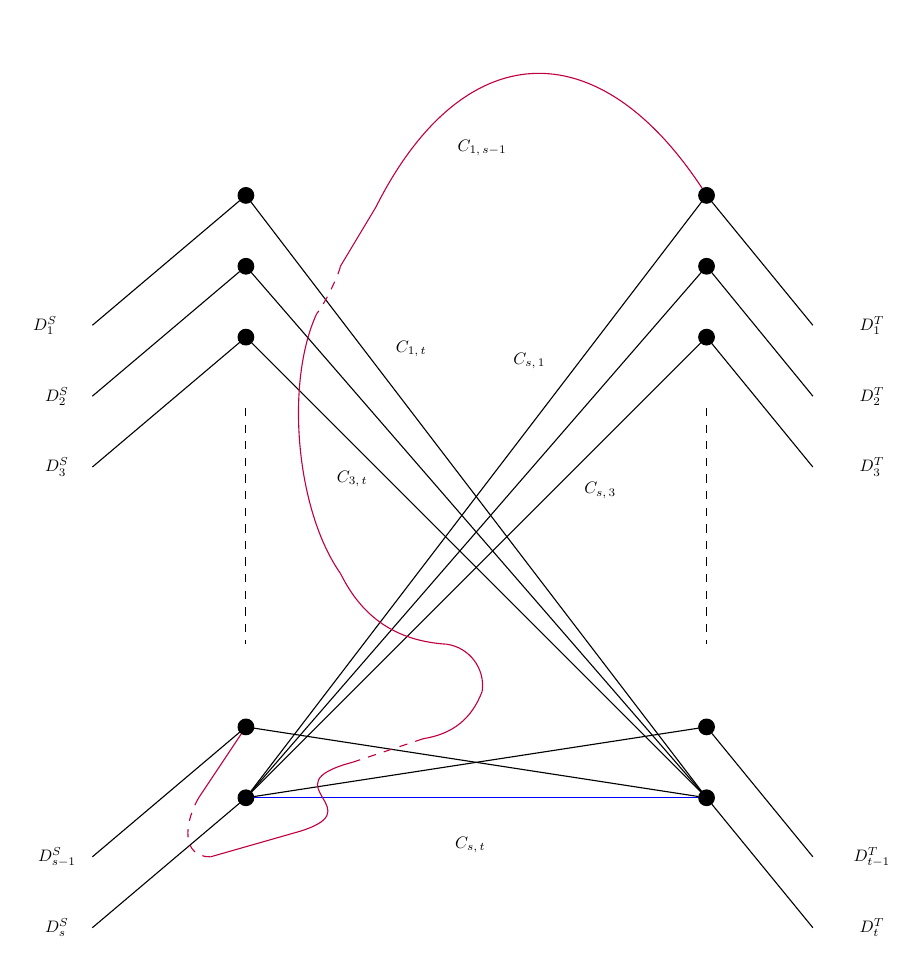
\begin{tikzpicture}[thick,scale=0.6, every node/.style={transform shape}]
	\begin{pgfonlayer}{nodelayer}
		\node [style=Filled Basic] (0) at (0.25, 9.25) {};
		\node [style=Filled Basic] (1) at (0.25, 7.75) {};
		\node [style=Filled Basic] (2) at (0.25, 6.25) {};
		\node [style=none] (3) at (0.25, 4.75) {};
		\node [style=none] (4) at (0.25, -0.25) {};
		\node [style=Filled Basic] (5) at (0.25, -2) {};
		\node [style=Filled Basic] (6) at (0.25, -3.5) {};
		\node [style=Filled Basic] (7) at (10, 9.25) {};
		\node [style=Filled Basic] (8) at (10, 7.75) {};
		\node [style=Filled Basic] (9) at (10, 6.25) {};
		\node [style=none] (10) at (10, 4.75) {};
		\node [style=none] (11) at (10, -0.25) {};
		\node [style=Filled Basic] (12) at (10, -2) {};
		\node [style=Filled Basic] (13) at (10, -3.5) {};
		\node [style=none] (24) at (-3, 6.5) {};
		\node [style=none] (25) at (-3, 5) {};
		\node [style=none] (26) at (-3, 3.5) {};
		\node [style=none] (27) at (-3, -4.75) {};
		\node [style=none] (28) at (-3, -6.25) {};
		\node [style=none] (29) at (12.25, 6.5) {};
		\node [style=none] (30) at (12.25, 5) {};
		\node [style=none] (31) at (12.25, 3.5) {};
		\node [style=none] (32) at (12.25, -4.75) {};
		\node [style=none] (33) at (12.25, -6.25) {};
		\node [style=none] (34) at (3, 9) {};
		\node [style=none] (35) at (2.25, 7.75) {};
		\node [style=none] (36) at (1.75, 6.75) {};
		\node [style=none] (37) at (2.25, 1.25) {};
		\node [style=none] (44) at (-3.75, 6.5) {};
		\node [style=none] (45) at (-3.75, 5) {};
		\node [style=none] (46) at (-3.75, 3.5) {};
		\node [style=none] (47) at (-3.75, -4.75) {$D_{s-1}^S$};
		\node [style=none] (48) at (-3.75, -6.25) {$D_s^S$};
		\node [style=none] (50) at (-3.75, 5) {$D_2^S$};
		\node [style=none] (51) at (-3.75, 3.5) {$D_3^S$};
		\node [style=none] (54) at (-4, 6.5) {$D_1^S$};
		\node [style=none] (55) at (13.5, 6.5) {};
		\node [style=none] (56) at (13.5, 5) {};
		\node [style=none] (57) at (13.5, 3.5) {};
		\node [style=none] (58) at (13.5, -4.75) {$D_{t-1}^T$};
		\node [style=none] (59) at (13.5, -6.25) {$D_t^T$};
		\node [style=none] (60) at (13.5, 5) {$D_2^T$};
		\node [style=none] (61) at (13.5, 3.5) {$D_3^T$};
		\node [style=none] (62) at (13.5, 6.5) {$D_1^T$};
		\node [style=none] (63) at (5.25, 10.25) {};
		\node [style=none] (64) at (5.25, 10.25) {$C_{1, \, s-1}$};
		\node [style=none] (65) at (12.25, -4.75) {};
		\node [style=none] (66) at (4.5, -0.25) {};
		\node [style=none] (67) at (5.25, -1.25) {};
		\node [style=none] (68) at (4, -2.25) {};
		\node [style=none] (69) at (2.5, -2.75) {};
		\node [style=none] (70) at (1.25, -4.25) {};
		\node [style=none] (71) at (-0.5, -4.75) {};
		\node [style=none] (72) at (-0.75, -3.5) {};
		\node [style=none] (73) at (3.75, 6) {$C_{1, \, t}$};
		\node [style=none] (74) at (2.5, 3.25) {};
		\node [style=none] (75) at (6.25, 5.75) {$C_{s, \, 1}$};
		\node [style=none] (76) at (7.75, 3) {$C_{s, \, 3}$};
		\node [style=none] (77) at (5, -4.5) {};
		\node [style=none] (78) at (5, -4.5) {$C_{s,\,t}$};
		\node [style=none] (79) at (2.5, 3.25) {$C_{3, \, t}$};
	\end{pgfonlayer}
	\begin{pgfonlayer}{edgelayer}
		\draw [style=Filled Blue] (6) to (13);
		\draw (6) to (12);
		\draw (5) to (13);
		\draw (2) to (13);
		\draw (1) to (13);
		\draw (0) to (13);
		\draw (6) to (9);
		\draw (8) to (6);
		\draw (7) to (6);
		\draw [style=Dashed Black] (3.center) to (4.center);
		\draw [style=Dashed Black] (10.center) to (11.center);
		\draw (24.center) to (0);
		\draw (25.center) to (1);
		\draw (26.center) to (2);
		\draw (27.center) to (5);
		\draw (28.center) to (6);
		\draw (33.center) to (13);
		\draw (9) to (31.center);
		\draw (8) to (30.center);
		\draw (7) to (29.center);
		\draw [style=Red, bend right=60, looseness=1.50] (7) to (34.center);
		\draw [style=Red] (34.center) to (35.center);
		\draw [style=Red, bend right, looseness=0.75] (36.center) to (37.center);
		\draw [style=new edge style 0, bend left=15, looseness=0.50] (35.center) to (36.center);
		\draw (12) to (65.center);
		\draw [style=Red] (5) to (72.center);
		\draw [style=Red] (71.center) to (70.center);
		\draw [style=Red, in=-165, out=15, looseness=2.50] (70.center) to (69.center);
		\draw [style=Red, bend right] (68.center) to (67.center);
		\draw [style=Red, bend left=45] (66.center) to (67.center);
		\draw [style=Red, bend left] (66.center) to (37.center);
		\draw [style=new edge style 0, in=-180, out=-120, looseness=1.25] (72.center) to (71.center);
		\draw [style=new edge style 0] (69.center) to (68.center);
	\end{pgfonlayer}
\end{tikzpicture}
}
\caption{Figure 2. This is currently not correct, fix the intersection}
\end{figure}
Hence if we choose a floating $-1$ curve $C_{u, \, v}$ to contract the only remaining floating curves are $C_{u, \, \beta}$ and $C_{\alpha , \, v}$ where $\alpha \in \{ 1, \dots, s\}$ and $\beta \in \{1 , \dots , t \}$. When the second floating curve is contracted this uniquely defines whether we are iterating over $s$ or over $t$. So after two contractions the cascade is uniquely defined. To see where it ends up we note that a basic surface is uniquely defined by the number of $-1$ curves coming out of each curve on the boundary. Picking one of these chains of  leads to either $s$ blowdowns or $t$ blowdowns. These cases behave symmetrically, so focusing on the case of $s$ blowdowns we get a curve $E_1 \subset Y$ with self intersection $a$ and no $-1$ curves coming out of it. So it is not unreasonable to hope that this admits a map to $\mb{F}_{a_1}$. To show this we introduce even more notation. 
We note that we can start by contracting all $-1$ curves intersecting the exceptional curves. We previously had $2$ fibers $F_1 = [f_1, \dots, f_{m_1}]$ and $F_2 = [g_1, \dots g_{m_2}]$ and after purely toric contractions $F_1$ can be mapped to $[-1, \, -2, \, -2 \dots -2 \, -1]$ with length $k_1$, the analogous statement holds for $F_2$. We note that the curve $E_1$ is still in the fiber $[-1, \, -2, \, -2, \dots -2, \, -1]$. After our new series of contractions we now have a curve configuration $[-a_1, \, f_2, \,f_3 \dots f_{m_1}, \, L-1-a_i, \, g_1, \dots g_{m_2}] = [-a_1, \, f_1,  \, f_2 \dots f_{m_1}, \, -k_1-k_2-1, \, g_1, \dots , g_{m_2}]$. We can repeat our toric contractions to contract this too $[-a_1, \, -2, \dots -2, \, -1, \, -k_1 -k_2 +1 , \, -1, \, -2, \dots , \, -2, \, -1]$, at this point as the number of $-2$ curves on the left is $k_1$ and the number of $-2$ curves on the right is $k_2$ we see that this curve configuration can be constructed by blowing up the configuration $[-a_1, \, 0]$ in the following way:
\[
% https://tikzcd.yichuanshen.de/#N4Igdg9gJgpgziAXAbVABwnAlgFyxMJZABgBoAmAXVJADcBDAGwFcYkRkBaegfQEZSAAgA6woZ3JDR4gSLGCJlEAF9S6TLnyEUZAMzU6TVuy69Z0hZLlQIOOIPFXOAa36dz890tXrseAkRkACwGDCxsiBzc-FKeVqI2dg4KrnwKgq7kCh6OsY7WtvaKKmogGH5agaR8oUYRUWZ52aQWXiW+mgE6pMS14SbROYK9KgYwUADm8ESgAGYAThAAtkgCIDgQSMQ+IAvLWzQbSLo7eyuIuoebiEGni+eS69d8ypTKQA
\begin{tikzcd}
{[-a_1, \, 0]}                                                          \\
{[-a_1, \, -1,\, -1]} \arrow[u]                                         \\
{[-a_1, \, -2, \, -1, \, -2]} \arrow[u]                                 \\
{[-a_1, \, -2, \dots , -2, -k_1-1, \, -1]} \arrow[u]                    \\
{[-a_1, \, -2, \dots , -k_1 - k_2 -1, \, -2, \, -2 \dots -2]} \arrow[u]
\end{tikzcd}
\]
So in particular this arises from a basic surface with $k_2 = 0$, $k_1 = 1$ and the strict transform of only one becoming an exceptional curve. This concludes the first case.

\textbf{Case 2}: The second case is $(i, \, j) = (1, \, 2)$. We do not spell this out in the same level of detail. Replicating the above arguments we see that we now get exactly the same curve configuration as in Figure 2 except now connecting the curves $E_1^S$ to $E_2^T$. So once again this leads to a set of two branching contractions. Once again this leads to a basic surface with $k_1 = 1$ and $k_2 = 0$. However this time there are two fibers that are now exceptional curves on $Y$. This proof follows from exactly the same logic as above.

\textbf{Case 3}: The final case is $(i, \, j) = (2, \, 1)$. This is symmetrical to case 2.

A crucial point in this proof is that each case behave independently of the others as two floating curves don't intersect each other only if they lie in the same case.

We note that if there are no $-1$ curves coming out of the curves $E_1^S$ and $E_1^T$ then the cascade is a straight line as the above discussion is entirely predicated on their existence. This concludes the cascade for basic surfaces of this type. 

We make a quick mention of what happens in the case where there is only one exceptional fiber. These surfaces all start by blowing up a point $k$ times. Label the exceptional curves that arose from blowing up this point $E_{k}, \dots E_1$ and we denote the strict transform of the fiber by $E_{0}$. Once again $L = a_1 -k+ 2$ and we have curves with self intersection $a_1 - i -1$ intersecting the $-1$ curves coming out of $E_i$. To get a $-1$ curve we need $a_1 - i - 1 < L = a_1 - k+2$ giving $k-i < 3$ so $i \in \{ k, \, k-1,\, k-2 \}$.  After $a_1-k$ blowups we get a straight chain of blowdowns arising from floating $-1$ curves intersecting $-1$ curves coming out of $E_k$. After $a_1-k+1$ blowups we also get $-1$ curves intersecting the fiber $E_{k-1}$. These curves, pre blowups, intersect the potential floating curves arising from $E_k$ $a_1 - k - 1?$ times. We have then blown up $a_1-k+1$ points 


\end{proof}
\begin{cor}
Let $S$ be a singularity with small discrepancy, $-a_1, \dots , -a_n$ be the self-intersection of the resolutions. Then if $n \geq \max (a_i) + 5 $. Then there exists no \ldp\ with only singularities of type $S$.
\end{cor}
\begin{rem}
It is fully possible for both $X_1$ and $X_2$ to exist but one of the $X_{a_i}^0$ to not exist. For example consider a singularity with resolution $-3, \, -8, \, -2, \, -2, \, -2, \, -2, \, -2, \, -2, \, -3$. There will be a surface $X$ such that the resolution will have a map to $\mb{F}_8$ but there will be no surface with a map from its resolution to $\mb{F}_3$.
\end{rem}


\section{Outside of the small discrepancy}

If you consider singularities of the type $\frac{1}{p}(1,1)$ we note that if $p \geq 7$ then a $\frac{1}{p}(1,1)$ singularity cannot be joined to any other $\frac{1}{p}(1,1)$ singularity by a $-1$ curve. Hence a similar analysis to  Theorem~\ref{ThmOnSing} gives us the bound that there cannot be a \ldp\ surface $X$ with singularities $\frac{1}{p_1}(1,1), \, \dots, \, \frac{1}{p_n}(1,1)$ and $p_1 \geq 7$ and more than 2 different singularities.

However when we enter the case where $p_1 < 7$ you can get surfaces with many more singularities. For instance consider the surface $X$ with the following minimal resolution:
\[
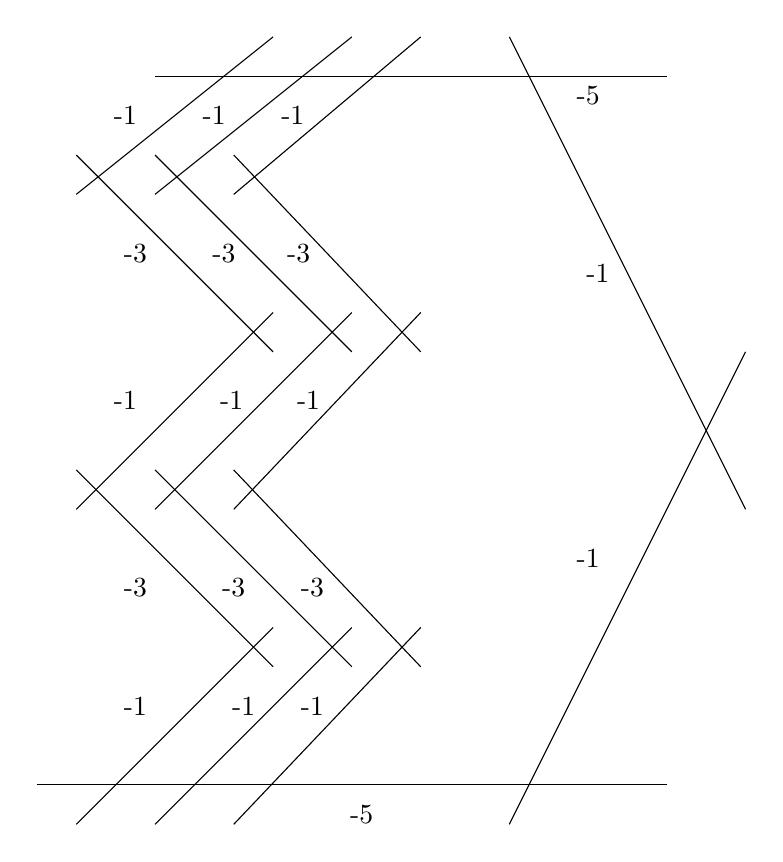
\begin{tikzpicture}[scale = 0.5]
	\begin{pgfonlayer}{nodelayer}
		\node [style=none] (0) at (-3, 3) {};
		\node [style=none] (1) at (10, 3) {};
		\node [style=none] (4) at (2, 4) {};
		\node [style=none] (5) at (-3, 0) {};
		\node [style=none] (6) at (3.75, 4) {};
		\node [style=none] (7) at (-1, 0) {};
		\node [style=none] (8) at (12, -8) {};
		\node [style=none] (9) at (6, 4) {};
		\node [style=none] (10) at (0, 4) {};
		\node [style=none] (11) at (-5, 0) {};
		\node [style=none] (12) at (-5, 1) {};
		\node [style=none] (13) at (0, -3) {};
		\node [style=none] (14) at (-3, 1) {};
		\node [style=none] (15) at (2, -3) {};
		\node [style=none] (16) at (-1, 1) {};
		\node [style=none] (17) at (3.75, -3) {};
		\node [style=none] (20) at (0, -4) {};
		\node [style=none] (21) at (2, -4) {};
		\node [style=none] (22) at (3.75, -4) {};
		\node [style=none] (23) at (-5, -7) {};
		\node [style=none] (24) at (-3, -7) {};
		\node [style=none] (25) at (-1, -7) {};
		\node [style=none] (26) at (-5, -8) {};
		\node [style=none] (27) at (-3, -8) {};
		\node [style=none] (28) at (-1, -8) {};
		\node [style=none] (29) at (-3.75, 2) {-1};
		\node [style=none] (30) at (-1.5, 2) {-1};
		\node [style=none] (31) at (0.5, 2) {-1};
		\node [style=none] (32) at (-3.5, -1.5) {-3};
		\node [style=none] (33) at (-1.25, -1.5) {-3};
		\node [style=none] (34) at (0.65, -1.5) {-3};
		\node [style=none] (35) at (-3.75, -5.25) {-1};
		\node [style=none] (36) at (-1.05, -5.25) {-1};
		\node [style=none] (37) at (0.9, -5.25) {-1};
		\node [style=none] (38) at (2.25, -5.5) {};
		\node [style=none] (39) at (0, -11) {};
		\node [style=none] (40) at (2, -11) {};
		\node [style=none] (41) at (3.75, -11) {};
		\node [style=none] (42) at (0, -12) {};
		\node [style=none] (43) at (2, -12) {};
		\node [style=none] (44) at (3.75, -12) {};
		\node [style=none] (45) at (-6, -15) {};
		\node [style=none] (46) at (-3, -15) {};
		\node [style=none] (47) at (-1, -15) {};
		\node [style=none] (48) at (-5, -16) {};
		\node [style=none] (49) at (-3, -16) {};
		\node [style=none] (50) at (-1, -16) {};
		\node [style=none] (51) at (-3.5, -10) {-3};
		\node [style=none] (52) at (-1, -10) {-3};
		\node [style=none] (53) at (1, -10) {-3};
		\node [style=none] (54) at (-3.5, -13) {-1};
		\node [style=none] (55) at (-0.75, -13) {-1};
		\node [style=none] (56) at (1, -13) {-1};
		\node [style=none] (57) at (10, -15) {};
		\node [style=none] (58) at (12, -4) {};
		\node [style=none] (59) at (6, -16) {};
		\node [style=none] (60) at (8.25, -2) {-1};
		\node [style=none] (61) at (8, -9.25) {-1};
		\node [style=none] (62) at (2.25, -15.75) {-5};
		\node [style=none] (63) at (8, 2.5) {-5};
	\end{pgfonlayer}
	\begin{pgfonlayer}{edgelayer}
		\draw (11.center) to (10.center);
		\draw (5.center) to (4.center);
		\draw (7.center) to (6.center);
		\draw (12.center) to (20.center);
		\draw (14.center) to (21.center);
		\draw (16.center) to (22.center);
		\draw (0.center) to (1.center);
		\draw (26.center) to (13.center);
		\draw (27.center) to (15.center);
		\draw (28.center) to (17.center);
		\draw (23.center) to (42.center);
		\draw (24.center) to (43.center);
		\draw (25.center) to (44.center);
		\draw (39.center) to (48.center);
		\draw (49.center) to (40.center);
		\draw (41.center) to (50.center);
		\draw (45.center) to (57.center);
		\draw (9.center) to (8.center);
		\draw (58.center) to (59.center);
	\end{pgfonlayer}
\end{tikzpicture}
\]
This has $h^0(-K_X) \neq 0$, $-K_X^2 = \frac{3}{5}$, six $\frac{1}{3}(1,1)$ singularities and two $\frac{1}{5}(1,1)$ singularities. In addition it admits no normal toric degeneration, as it is a complexity one surface and hence any degeneration would have to be equivariant. We can construct this as a toric complete intersection via cox rings and we see that it lies as a complete intersection in the toric variety given by the GIT quotient
\[
\begin{blockarray}{cc cc cc cc cc c}
	T_1 & T_2 & T_3 & T_4 & T_5 & T_6 & T_7 & T_8 & T_9 & T_{10} & T_{11} \\[4pt]
      \begin{block}{(cc cc cc cc cc c)}
	0&3&-6&-2&1&0&0&0&0&0&0 \\
	0&2&-4&-1&0&1&0&0&0&0&0 \\
	1&-2&3&0&0&0&0&0&0&0&0 \\ 
	0&3&-6&0&0&0&-2&1&0&0&0 \\ 
	0&2&-4&0&0&0&-1&0&1&0&0 \\
	0&-3&7&1&0&0&1&0&0&1&0 \\
	0&1&-2&0&0&0&0&0&0&-1&1 \\
      \end{block}
\end{blockarray}
\]
with the equations 
\[
\begin{array}{c}
T_1 T_2^2 T_3 + T_4 T_5^2 T_6 + T_7 T_8^2 T_9 \\[4pt]
T_1 T_2^2 T_3 + T_4 T_5^2 T_6  + \lambda T_{10} T_{11}
\end{array}
\]
We note that there are also surfaces which admit toric degenerations with the same numerics.
\end{document}